%\title{Kinematik Delta Roboter}
%\subtitle{Ergänzende Veranstaltung Vertiefungsprojekt 2}
%\author{Manuel Ilg}
%\maketitle

\begin{titlepage}
	\setlength{\TPHorizModule}{\paperwidth}
	\setlength{\TPVertModule}{\paperheight}
	
	\begin{textblock}{0.3}[0.1,-0.5](0.68,0.03)
	\makebox{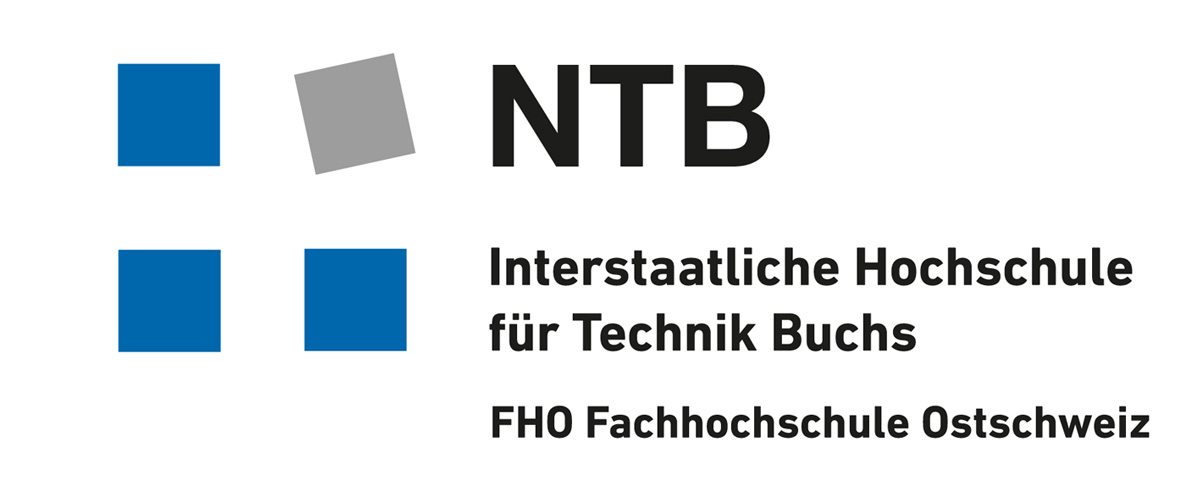
\includegraphics[width=5.5cm]{images/ntb_logo.jpg}}
	\end{textblock}
	\begin{textblock}{0.95}[0.1,-1.74](0.73,0.04)
	\makebox{
\includegraphics[width=5.5cm]{images/eeros_logo.png}}
	\end{textblock}
	\begin{textblock}{0.95}[0.4,-1.5](0.5,0.04)
	\makebox{
\includegraphics[width=5.5cm]{images/ros_logo.png}}
	\end{textblock}

	
%	\begin{textblock}{0.95}[0.1,-1.3](0.73,0.04)
%	\makebox{
\includegraphics[width=5.5cm]{images/ros_logo.png}}
%	\end{textblock}
%	\begin{textblock}{0.3}[0.1,-0.5](0.68,0.03)
%	\makebox{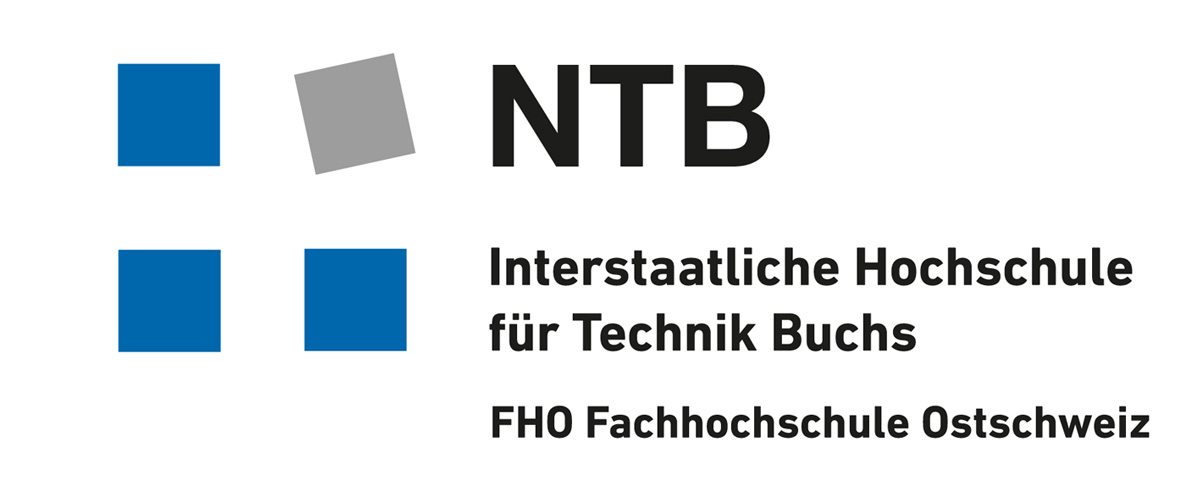
\includegraphics[width=5.5cm]{images/ntb_logo.jpg}}
%	\end{textblock}
    \vspace*{8cm}
    \begin{center}
    	\Huge{\color{HeadBlue}{ROS als unterstützendes Werkzeug für EEROS-Applikationen\\}}
		\vspace*{2cm}
		\normalsize
      	{\color{HeadBlue}{\sffamily{
      		\textbf{Vertiefungsarbeit 2} \\
      		\vspace*{1cm}
      		von \\
      		\vspace*{1cm}
%			~\newline
      		\textbf{Manuel Ilg} \\
      		\vspace*{0.1cm}
      		\textbf{manuel.ilg@ntb.ch}
      		}}}\\
		\vspace*{2cm}      	
%		\includegraphics[height=4cm]{images/logo_valens}

    \vspace*{3cm}
    \color{HeadBlue}
    \begin{tabular}{p{4cm}l}
      Referenten: & Prof. Einar Nielsen, Prof. Vincenzo Parisi \\
      Abgabedatum: & 27. August 2017
    \end{tabular}\\
    \end{center}
\end{titlepage}
